\section{Battery Management System}
\label{sec:BMSHWChapter}
The purpose of the BMS is to observe and make sure that the propulsion battery is kept within a safe operation area (SOA) at all times. It does this by monitoring cell voltages, temperature and current from the battery. The data the BMS collects from these units is compared to lower and upper threshold limits that are in compliance with the requirements from the Shell Eco-Marathon committee \footnote{See "sem-2016-global-rules-chapter1-010715"}. In case an event occurs where the temperature, cell voltages or current from the battery exceed the allowed thresholds, then the BMS must autonomously make sure to protect the rest of the vehicle from over-current by isolating the battery. \\
One can find a vast variety of commercially available BMSs that can fulfil the most of the requirements given by the Shell Eco-Marathon committee. However, not all of the BMSs are in compliance with these terms. An option of buying a fully functioning BMS and implementing a few things to meet the requirements is a possible solution. Nonetheless, most of these off-the-shelf BMSs are very power hungry and are usually meant for bigger systems with huge cell counts. However, a centralized and small BMS system is made, which is designed to be as energy efficient as possible. Furthermore, advanced features has been included such as the capability to measure State of Charge (SOC) and State of Health(SOH). The reason and argument for building the BMS as eco-friendly as possible is that it's crucial both power consumption and weight wise, when competing to be the most energy efficient team in our respective class. The lower the power consumption each unit has in the vehicle then e.g. a lower weighted battery can be used, which has less capacitance. Instead of a heavy and bulky battery.\\

\begin{figure}[H]
	\centering
	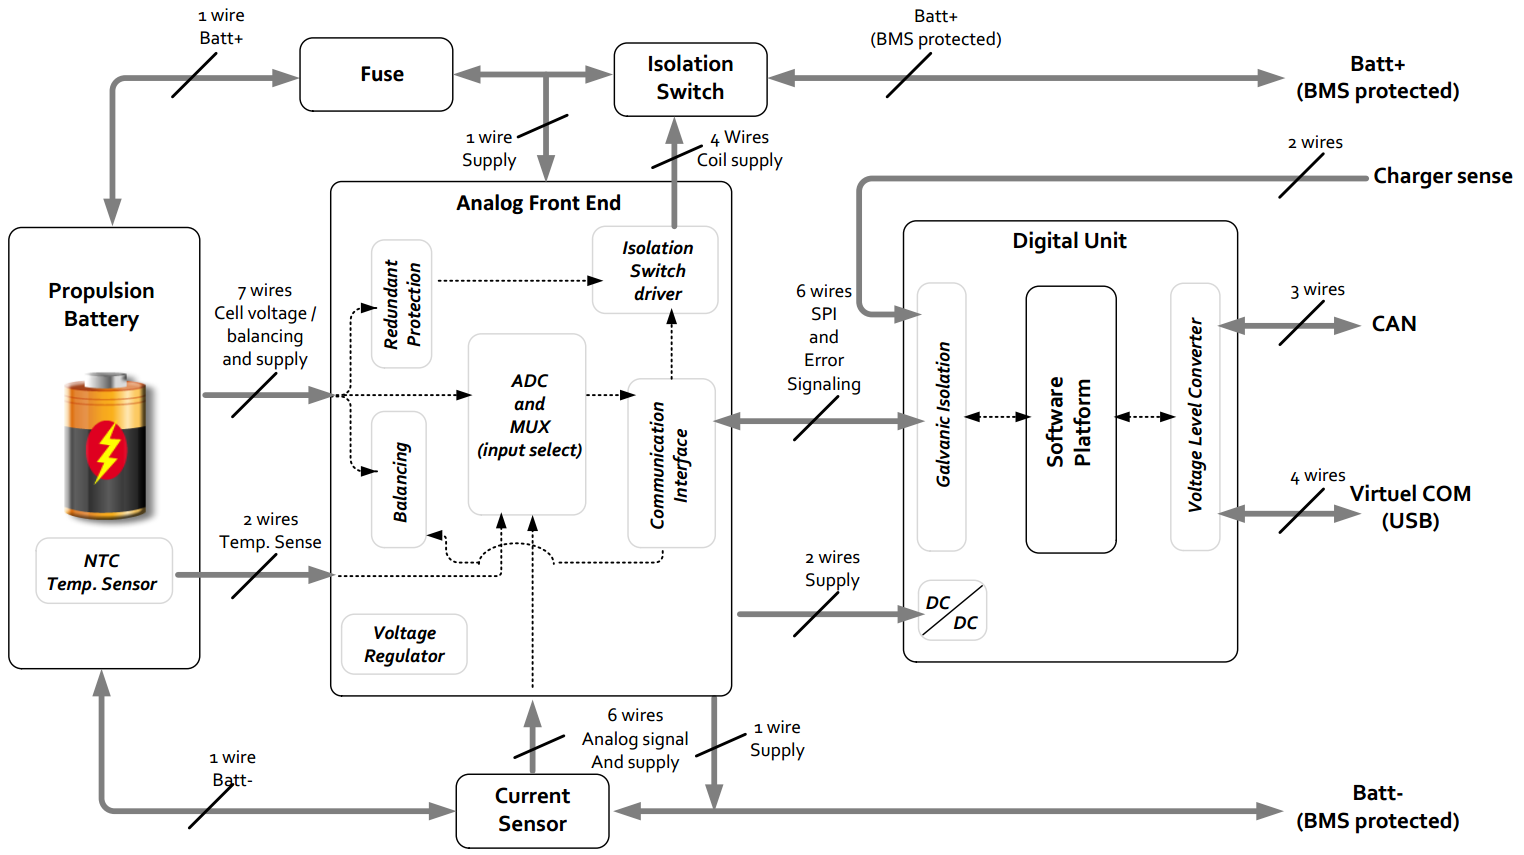
\includegraphics[width=1.0\linewidth]{Hardware/Pictures/BMSOverview}
	\caption[Empty]{An elaborated system and interfacing diagram for the BMS\footnotemark}
	\label{fig:BMSOverview}
\end{figure}
\footnotetext{Reference to 2013BMS sec 2.4\fxnote{Reference to 2013BMS Documentation sec 2.4}}

On figure \ref{fig:BMSOverview} you can see an overview of the BMS's interfaces and how it is connected to the rest of the vehicle. A truly detailed and descriptive IBD of the BMS has also been developed, which can be seen on figure \ref{fig:IBD_BMS}.

\subsection{Disclaimer}
In this chapter a detailed documentation of the BMS' hardware will be given. Furthermore, each unit contained in the BMS will be elaborated where the implementation and contents of each unit's circuitry is viewed upon as a black-box. This means that the units will be considered purchased from a third party vendor and therefore a  description of the circuitry will not be given. This will lead to a different form of documentation with a lot of references to the "manufacturer's" documentation that is the "BAC-projekt\_BMSogbatteri\_2013", which was developed by Jonas Nyborg in 2013. \fxnote{Reference to 2013BMS Documentation} documentation.\\
Thus in this chapter each of these units on figure \ref{fig:BMSOverview} will be elaborated, which means the general purpose and overview of each unit will be thoroughly documented. 

\subsection{Propulsion battery}
\label{sec:BMSBattery}
The purpose of this block is to deliver electrical energy to supply the Propulsion Motor as well as the rest of the systems in the vehicle.

This unit consists of twelve battery cells, which are responsible for storing electrical energy. Moreover, it must be capable of delivering the required current to turn the propulsion motor and be able to acquire energy from an external charger.   
The requirements for batteries when participating in the SEM are that the Prototype: battery electric class must utilize lithium type batteries. There was two choices between lithium type batteries: LiFePo4 and Lithium-ion polymer(Li-Po). Based on the tests done by Jonas \fxnote{REFERENCE to BMS "see Battery cell type test.pdf"} the Li-Po is the obvious choice, since it has a more satisfying capacity at the simulated worst case Eco-Marathon conditions. Moreover, it has a solid low internal resistance and weight for the purpose, whilst it can pack a lot of energy, alas it is very energy dense.\\
Since the Li-Po batteries are the better choice compared to the LiFePo4 batteries there will be used two Li-Po batteries in series to power the vehicle as required by design choices. Each of the batteries will have 6 cells, which results in a nominal voltage of 44.4V since each cell's nominal voltage is 3.7V. By doing so we are still within our limitations of not having the voltage exceed the maximum of 48V nominal as specified by AU2\_NF3. See section: \ref{sec:requirements}.\\
The batteries which have been purchased are of different capacities, however, they all have the same amount of cells, thus the same nominal voltage. This is done in preparation to test the required capacity needed by the vehicle. Furthermore, to be able to have a battery, which weighs less if the given capacity is more than enough for a run then that will improve the effectiveness of the car, since the motor will have less weight to pull.\\

\begin{figure}[H]
	\centering
	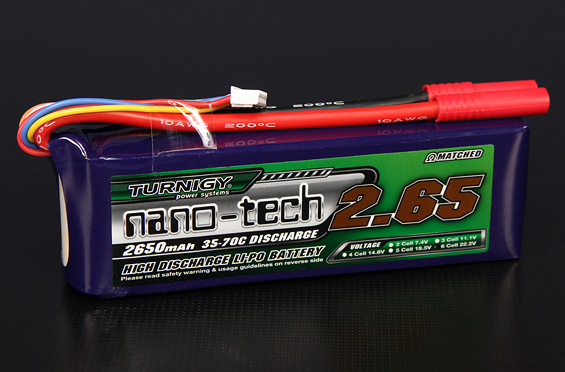
\includegraphics[width=0.6\linewidth]{Hardware/Pictures/2650battery}
	\caption[Empty]{Picture of the battery with 2650mAh\footnotemark}
	\label{fig:2650battery}
\end{figure}
\footnotetext{\url{http://www.hobbyking.com/hobbyking/store/__32651__Turnigy_nano_tech_2650mAh_6S_35_70C_Lipo_Pack_EU_Warehouse_.html} (Date: 20-05-2016)}

\textbf{Battery specifications}\\
Chemistry: Lithium-ion polymer(Li-cobalt)\\
Manufacturer: Turnigy\\
Type: Nano-tech\\
Nominal: 44.4V\\
Max. charging voltage: 50.4V\\
Min. voltage: 36V\\
Capacity: 2200 / 2650 / 3300mAh (depends on weather and achieved efficiency)\\
Max. continuous discharge: 35 / 35 / 45C\\
Max. charge rate: 8 / 8 / 10C\\
Weight: 730 / 834 / 1130g\\

\subsection{Analog Front end}
The purpose of this unit is that it performs calculations and analog to digital conversion of the battery's cell voltages, battery's temperature and the signal from current sensor. Moreover, this unit manages cell balancing on request from the digital unit. It also has additional battery protection independent of the digital unit.
An overview of the Analog Front End can be seen on figure \ref{fig:frontendOverview}.

\begin{figure}[H]
	\centering
	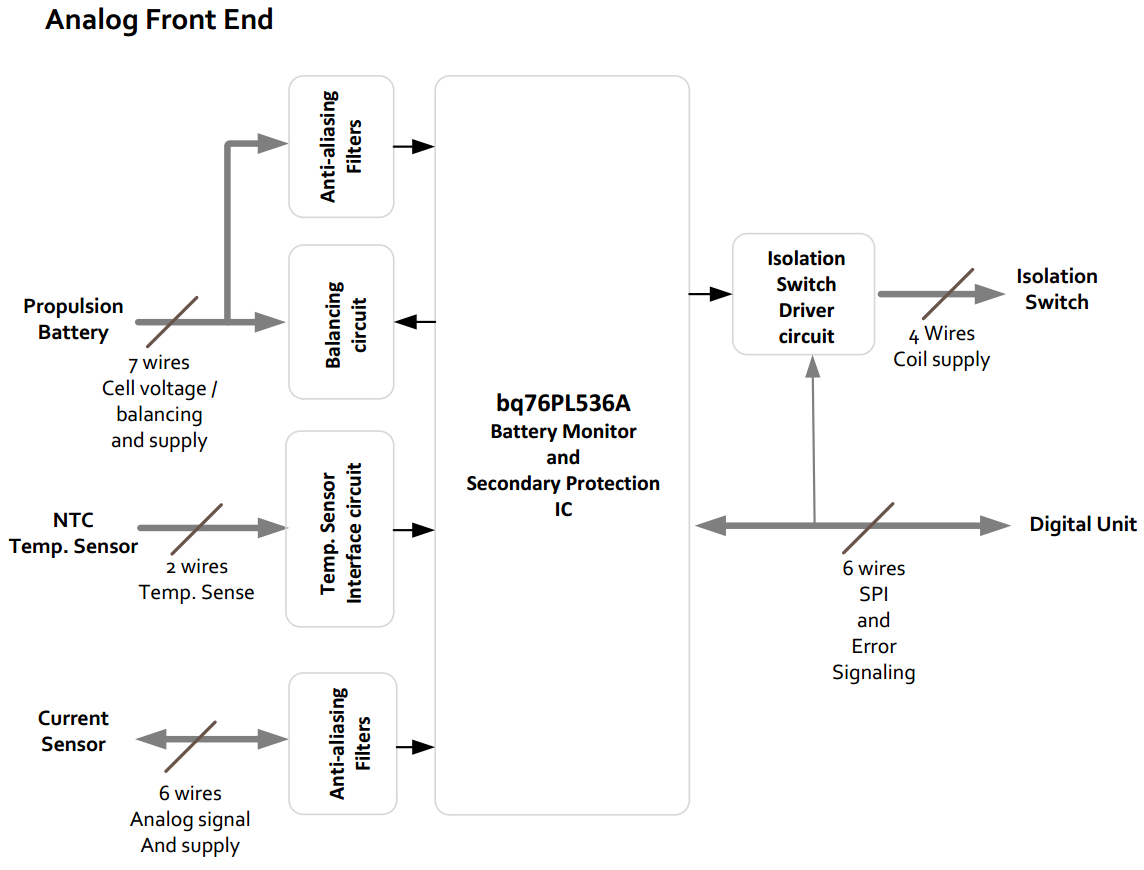
\includegraphics[width=1.0\linewidth]{Hardware/Pictures/analogfrontendOverview}
	\caption[Empty]{Analog Front End circuit blocks\footnotemark}
	\label{fig:frontendOverview}
\end{figure}
\footnotetext{Reference to 2013BMS\fxnote{Reference to 2013BMS Documentation}}

Now every circuit block will be elaborated on its functionality and how it all functions. If you wish to receive an even more thorough and detailed explanation, calculations and choices for components included, on the Analog Front End please see the \fxnote{reference to BMS2013 documentation}\\

\subsubsection{Anti-aliasing filters and cell balancing}
The anti-aliasing filters are there to decrease unwanted AC noise and they're placed very near their respective ADC inputs. The filters are traditional 1. order RC low-pass filters and they are implemented with respects to the battery monitor IC, which will be discussed in a moment.\\
The balancing circuit is connected to the battery monitor IC where it has outputs that are capable of controlling balancing of the cells. This process can be initialized by the Digital Unit if given parameters exceed a specific threshold.

There are two different instances where the cells can be balanced. This can be done either by connecting a charger to handle the balancing of the cells - this includes both discharging and charging. However, when no charger is connected the cells can only be balanced by discharging the individual cells.

ways that the circuit can  the cells  when it is connected to a charger to balance them by discharging them into bleeder resistors located on the circuit. This is done to keep the cells within the recommended safe operation area, which is in between 3-4.2V.



\subsubsection{Battery Monitor IC}
The heart of the BMS is the bq76PL536A-Q1 Battery Monitoring IC (new chip used since 2014 instead of the one on figure \ref{fig:frontendOverview}). It was chosen as it offers very low quiescent current, secondary protection, high precision voltage measurements and has the choice of stacking several IC's to attain support of a respective number of cells. The core functionality of this said chip is that it can receive and handle a lot of commands at the same time. As you see on figure \ref{fig:frontendOverview} it is connected to several circuits. It's job is, among other things, to receive a vast amount of data from it's surroundings / connected circuits. Example of data could be data requests from the Digital Unit, cell voltages, current sensor signal, cell temperature signal balancing requests from the Digital unit and more. With all of this data the Battery Monitoring IC converts this data through its ADC's where it sends them off to the Digital Unit. It can also perform the balancing if it receives a request. Furthermore, it is possible for it to drive the Isolation Switch, which means that in an event where the safe operation area is exceeded, it can cut off the power from the battery supply to the rest of the vehicle.

\subsubsection{Temperature sensor}
\fxnote{Evt. lave referencer til hvert eneste kapitel i BMS, ellers bare referere til et stort afsnit i starten også lade det være det. Også selvfølgelig referere billeder og ting taget fra rapporten.}
The temperature sensor is rather self explanatory, its purpose is to measure the temperature of the batteries. To do this a Thermistor(NTC) has been used to get voltage readouts by converting the temperature from the Thermistor. The temperature thresholds are specified in AU2\_F14, which can be seen here: \ref{sec:requirements}. If the given threshold is exceeded the Isolation Switch will prevent current from flowing through it.

\subsubsection{Isolation Switch Driver circuit}
The purpose of this part is to assure and allow the Battery Monitor IC and Digital Unit to control the Isolation Switch. In case of a parameter exceeding a threshold this is how the BMS shuts of current to the rest of the vehicle - By using the Isolation Switch Driver circuit.

\subsection{Analog Front End: Extension Module}
The Extension Module unit's purpose is that it gives the BMS the capability to support a larger amount of battery cells. Since the BMS Front End only supports 6 cells - and using the Extension Module the BMS can support up to 18 cells. This is done by stacking the Battery Monitor ICs - See figure \ref{fig:BMSextensionmod}. The Extension Module resembles the Analog Front End, however, it doesn't include the same features. Features like SPI to the Digital Unit, current sensor input and Isolation Switch Driver are left out and not included. It's purpose is to communicate with the Battery Monitor IC and report the voltages from the other cells. That way the BMS has full control and is able to monitor all the batteries.\\

\begin{figure}[H]
	\centering
	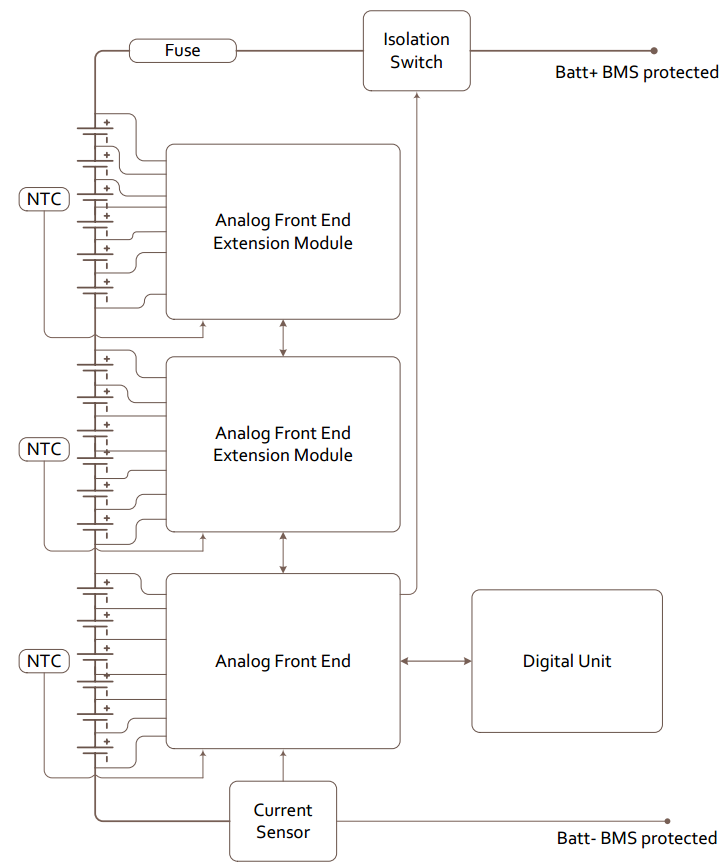
\includegraphics[width=1.0\linewidth]{Hardware/Pictures/BMSextensionmod}
	\caption[Empty]{Connection of Extension Modules\footnotemark}
	\label{fig:BMSextensionmod}
\end{figure}
\footnotetext{Reference to 2013BMS\fxnote{Reference to 2013BMS Documentation kap 3.1.3}}

On figure \ref{fig:BMSextensionmod} you can see an overview of how a possible stacking of Battery Monitor ICs can be handled. You can also see that only the Analog Front End has a connection to the Digital Unit through SPI.\\
The fuse block seen on figure \ref{fig:BMSextensionmod} is a fast-acting fuse that can handle up to 30A before it breaks. It is implemented as a requirement by the Shell Eco-Marathon committee.\\
A few things to note on this diagram: The extension modules are capable of utilising an NTC Thermistor, however, for simplicity it has been chosen that only the Analog Front End contains and handles the Thermistor to measure the temperature of the batteries. One of these is more than enough since the other Thermistors would simply put out almost or exactly the same readings.

\subsection{Current Sensor}
The purpose of this unit is to measure the amount of current flowing through the sensor as well as the direction of the current. The data that the sensor generates is sent to and handled by the Analog Front End. \\
The choice for a current sensor was either to use a Hall current sensor as done in the Motor Controller unit or use a shunt current sensor. Since the goal is to make the BMS as energy efficient as possible the choice fell on the shunt based sensor. It is a better choice when considering the power consumption for the current sensor, more on the specifications and calculations can be found in xx \fxnote{reference BMS 2013 sec 3.1.4}.

\subsection{Isolation Switch}
The Isolation Switch has a very important functionality concerning the BMS. If anything goes wrong with the battery, which means it exceeds the safe operation area of any specified thresholds, then the Isolation Switch will prevent any current from flowing through it and to the distribution block. \\
Since it is a requirement by the Shell Eco-Marathon committee that an automatic form of isolation of the battery from the rest of the system is required within the BMS. This leaves us with the only choice of using a relay to fulfil this requirement. Nonetheless, a relay isn't the best solution when considering low power application and consumption. If the BMS was to be implemented in a commercial application where it wouldn't be obligatory to fulfil the Shell Eco-Marathon committee's requirement, then a solution using RDS MOSFETs would be a huge benefactor when considering supply current draw.\\
The Isolation Switch relay is of a type Normally Open(NO), which means unless it has a specific amount of voltage running through it's coils, then it won't allow current to flow through it's terminals. Nonetheless, the relay is  capable of withstanding a current of up to 30 Amps and has a nominal coil rating of 48V, which is within the specified ratings by Shell's rules. Below on figure \ref{fig:BMSRelay} the physical relay can be seen.

\begin{figure}[H]
	\centering
	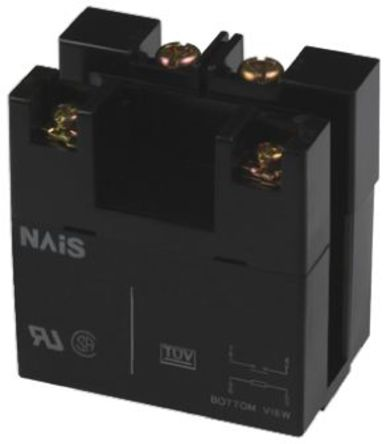
\includegraphics[width=0.3\linewidth]{Hardware/Pictures/BMSRelay}
	\caption[Empty]{Picture of the Isolation Switch Relay used in the BMS\footnotemark}
	\label{fig:BMSRelay}
\end{figure}
\footnotetext{\url{http://uk.rs-online.com/web/p/non-latching-relays/6995676/} (Date: 21-05-2016)}

The Isolation Switch works by having the Digital Unit send commands to the Analog Front End, which in return controls the Isolation Switch Driver. And the driver controls the relay. If the cells are within a safe operation area and the Digital Unit hasn't told the Analog Front End to open the relay - meaning to prevent current flowing through it - then a secondary option is available to isolate the battery manually. This functionality is implemented by a Emergency Switch(button). It serves the purpose of delivering a 0V drop over the relay's coil when the Emergency Switch is pressed. This will force the relay to open and seize to supply current through its terminals and therefore isolate the battery.

\subsection{Digital Unit (HW)}
This unit's purpose is to gather the measured values from the Analog Front End and thereafter run calculations and approximations of cell and battery parameters. If any of these parameters exceeds a specific threshold then the Digital Unit is capable of utilizing the Isolation Switch to prevent damages to the rest of the vehicle's system. The Digital Unit is capable of communication with external units. Furthermore, the Digital Unit utilizes galvanic isolation and a DC/DC converter, which will be described in detail below. 

\begin{figure}[H]
	\centering
	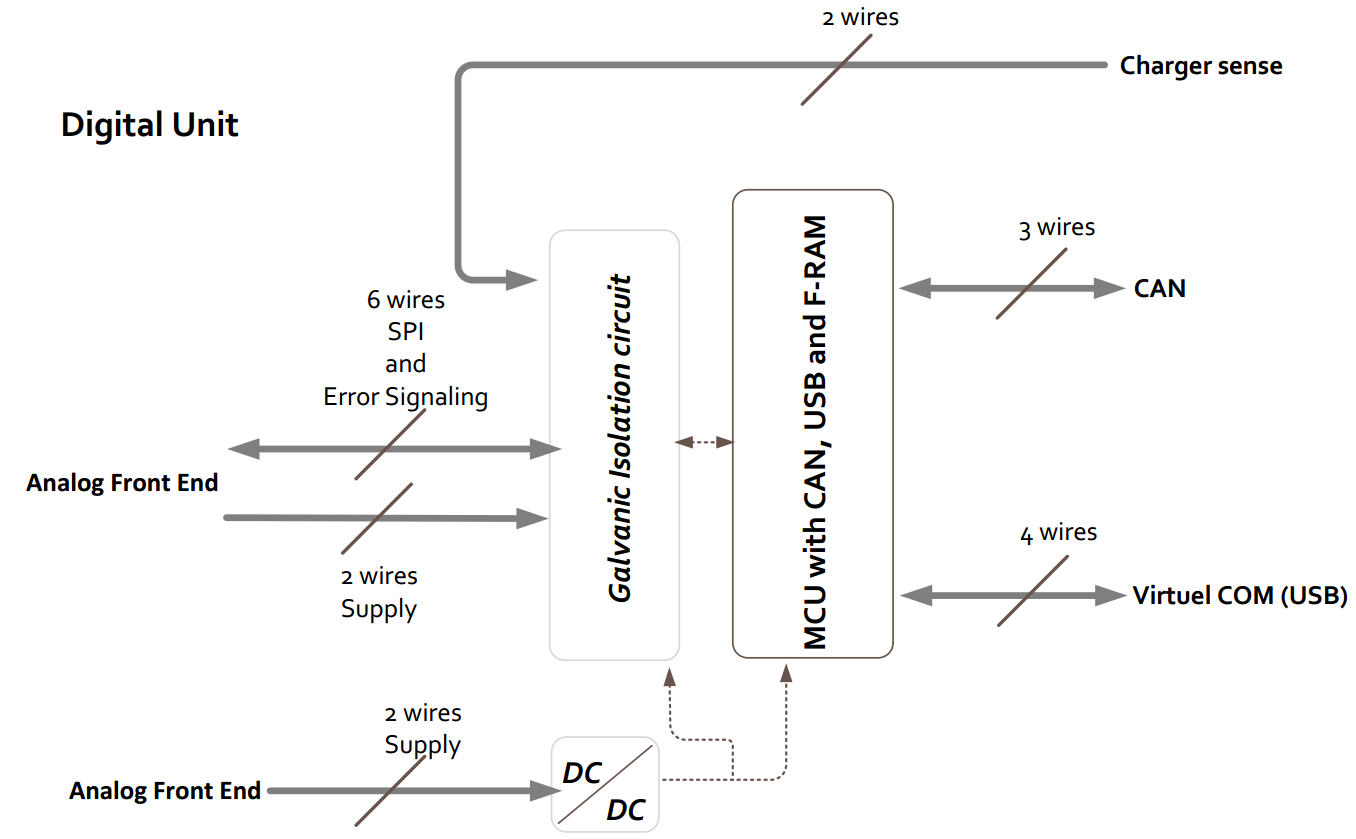
\includegraphics[width=1.0\linewidth]{Hardware/Pictures/BMSdigitalUnit}
	\caption[Empty]{Digital Unit circuit blocks\footnotemark}
	\label{fig:BMSdigitalUnit}
\end{figure}
\footnotetext{Reference to 2013BMS\fxnote{Reference to 2013BMS Documentation kap 3.1.6}}

On figure \ref{fig:BMSdigitalUnit} you can see the Digital Unit and its contents. A elaborative description will be given on each of the circuit blocks in this section. As mentioned earlier none of the implementation will be addressed since this unit along with others are viewed upon as a black box.

\subsubsection{Galvanic Isolation}
Galvanic isolation is a principle of isolating functional parts of electrical systems to prevent flow of current. This means that no direct path of conductivity is permitted. However, information can still be exchanged by utilization of different techniques such as electromagnetic waves or by optical and mechanical means. These are simply a few methods mentioned, there are a lot of various ways to transmit information by using galvanic isolation.\\
In any case, the way the galvanic isolation is used in the BMS is through the use of optocouplers. Optocouplers or opto-isolators are components that by the use of light can transfer electrical signals between two isolated circuits. This application often consists of an LED on the sender side, and a photodiode on the receiver side - You can see figure \ref{fig:BMSoptocoup} for a quick orientation of the principle.

\begin{figure}[H]
	\centering
	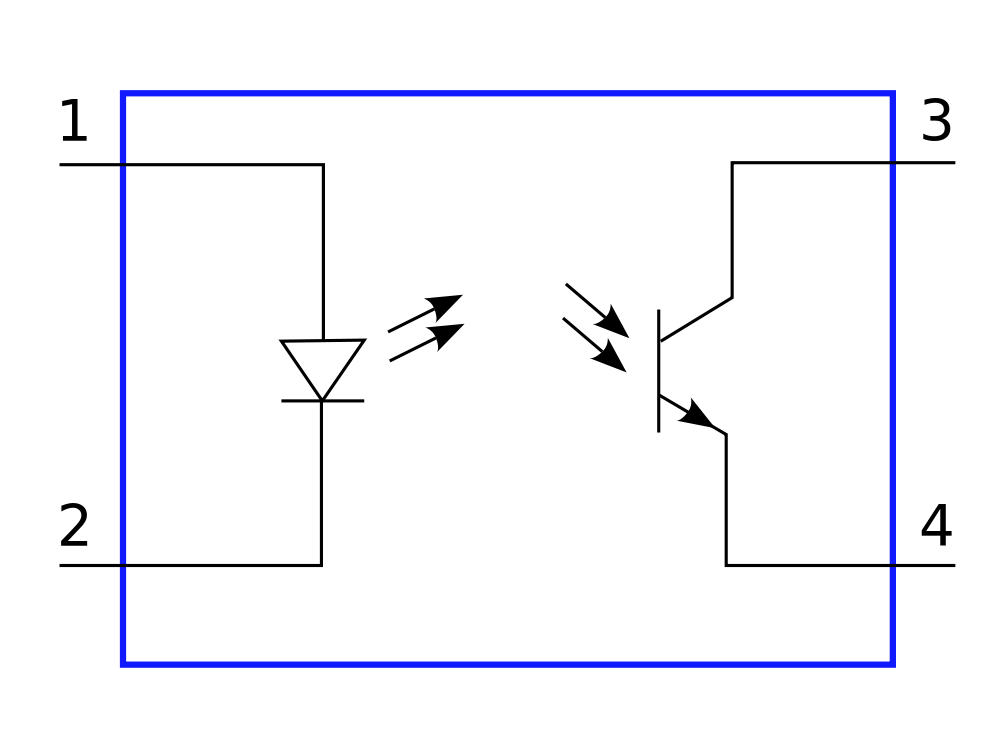
\includegraphics[width=0.5\linewidth]{Hardware/Pictures/BMSoptocoup}
	\caption[Empty]{Basic illustration of the functionality of an optocoupler\footnotemark.}
	\label{fig:BMSoptocoup}
\end{figure}
\footnotetext{\url{https://commons.wikimedia.org/wiki/File:Optocoupler.svg} (Date: 22-05-2016)}

When the sender side wants to send something it activates the LED. The light from the LED activates the photodiode on the other side of the isolated circuit. Then through either OP-AMPs or transistors the light received in the photodiode can be translated into electrical signals and thus you utilize light to send information. Other than being able to send information through light, the optocouplers are also good for safety. They can often withstand high input-to-output voltages and voltage transients. \\
With low power consumption in mind, a few digital isolators based on optocouplers were examined to find the best possible solution. You can see more about which digital isolators were investigated in the \fxnote{reference to BMS2013 sec 3.1.6.1}. The examination of the two digital isolators resulted in neither of them being chosen since they were consuming to much power on both the receiver and sender side. Therefore the Galvanic Isolation circuit is based on dual-channel optocouplers. This design approach makes it possible to have a low power consumption during use and nearly nothing while quiescent. Furthermore, when the SPI bus isn't used for non-isolated devices a smart power saving option has been implemented, more on this can be found in \fxnote{BMS2013 reference cap 3.1.6.1}.

\subsubsection{DC/DC Converter}
The purpose of the DC/DC Converter is to convert the battery voltage, which is expected to be around 44.4V nominal, to a lower voltage that is usable by the other components in the Digital unit. This includes the Galvanic Isolation and micro controller circuit with its included parts. \\
Since power consumption is a very important factor in the design of the BMS, several DC/DC converters were examined to see if it was possible to find a suitable prefabricated and commercial DC/DC converter. The results of this inspection and a more detailed description of the converter can be found in \fxnote{reference to BMS2013 sec 3.1.6.2}. Moreover, please note that a newer DC/DC Converter than in the 2013 BMS Documentation has been used - More details on the changes done since the 2013 documentation can be found in section \fxnote{reference to CHANGES from BMS 2013 to BMS 2014}.  

\subsubsection{MCU with CAN, USB and F-RAM}
This unit is the brains of the operation. It consists of vital parts to make the BMS function properly. It has a micro controller that has an implemented CAN controller. It also has non-volatile memory, which is in the form of Ferroelectric Random Access Memory (F-RAM). Nonetheless, a USB interface is also part of this unit, which makes it possible to directly debug the BMS through the micro controller. For more info on how to use the USB interface and how to program the BMS see section \ref{sec:BMSDebugging}.

\textbf{The MCU - AVR-CAN}\\
The micro controller unit is a OLIMEX AVR-CAN development board. It would have been sufficient to have emulated a CAN interface. However, the platform is now equipped for future improvements by using a micro controller with an integrated CAN controller. This way a CAN protocol is required for the BMS if it is to become commercially viable.

\begin{figure}[H]
	\centering
	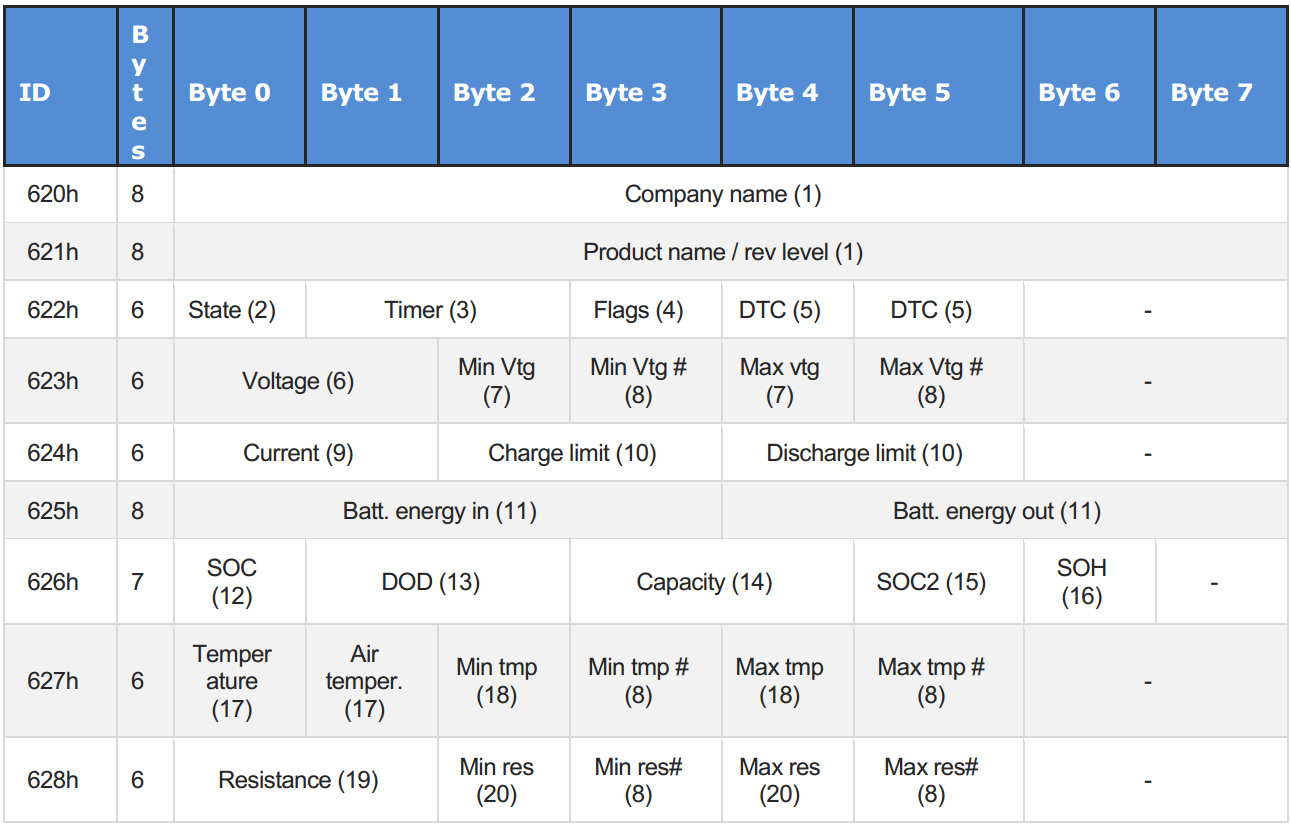
\includegraphics[width=1.0\linewidth]{Hardware/Pictures/BMSCANProto}
	\caption[Empty]{CAN protocol for the BMS\footnotemark}
	\label{fig:BMSCANProto}
\end{figure}
\footnotetext{Reference to 2013BMS\fxnote{Reference to 2013BMS Documentation kap 1.5.3.1}}

On figure \ref{fig:BMSCANProto} you can see the CAN protocol, which is based on the Original Standard Traction Pack. Since the BMS was first implemented with a CAN bus it was found that it would be a good idea to perform heavy duty data logging on the Motor Controller via CAN bus, therefore a CAN transceiver and software to support it was implemented on the Motor Controller. For more info about the Can-transceiver see section \ref{sec:CAN-Tranceiver}. A more detailed description of the CAN protocol can be found in \fxnote{reference to BMS2013}.\\
Otherwise the AVR-CAN is mainly used as a control unit, since it performs calculations and sends commands to the Analog Front End all whilst monitoring different thresholds for safe operation areas for the batteries. The AVR-CAN is mainly used for programming and this is where all the BMS Software is stored and executed by the AT90CAN128 IC which is contained on the developer board. The software functionality will be described in the BMS Software chapter \fxnote{Godt med krydsreferencer til forskellige dokumenter - burde være include(xr) ... ?} %\externaldocument{BMSSoftware}.. 

\textbf{F-RAM}\\
As mentioned earlier it was required by the 2013 requirements (BMS\_F.5)\fxnote{reference BMS 2013 sec 1.5.1.2.} that the BMS must be able to store the most critical information on internal memory for the ability to read the data on the USB interface or SD-card on the Motor Controller. Since the AVR-CAN module didn't have enough on-board memory a few options were considered for implementing a solution. EEPROM was considered since it is non-volatile and cheap but offers a limited amount of write cycles as well as the power consumption is fairly higher than the  F-RAM. However, the solution is F-RAM, which is non-volatile has a lot of write cycles and is fairly low power between write cycles. Moreover, please note that a newer F-RAM module than in the 2013 BMS Documentation has been used - More details on the changes done since the 2013 documentation can be found in section \fxnote{reference to CHANGES from BMS 2013 to BMS 2014}.  

\subsection{Unit test}
In this section a description of each of the elaborated units will be given below. 

\subsubsection{Isolation Switch}
The way this unit was tested is rather straight forward. A few things were used to complete it. These include a digital multimeter and a power supply. This test is both audible and visual. To test it the datasheet \fxnote{reference to RELAY datasheet} for the relay was read to make sure the coil voltages were known beforehand. It is expected that the pick-up voltage is 70\% or less of the nominal coil voltage, which is 48V for our Isolation Switch relay. Whereas the drop-out voltage is expected to be around 10\% of the nominal coil voltage. This translates to a pick-up voltage of max 33.6V and a drop-out voltage of max 4.8V.\\
When the test was done a voltage drop over the coil was driven by the power supply. We kept increasing the voltage drop until one of two things happened. Either the digital multimeter made a sound, which it will when it achieves continuity. Or one could hear the relay click, which means that the pick-up voltage was reached.\\
From the test done a pick-up coil voltage of approximately 23V was reached as well as a drop-out voltage of approximately 12V. Below on figure \vref{fig:BMSIsoTest} you can see the test setup for the test. Where the voltage was read from the power supply whilst the multimeter was checking for continuity. 

\begin{figure}[H]
	\centering
	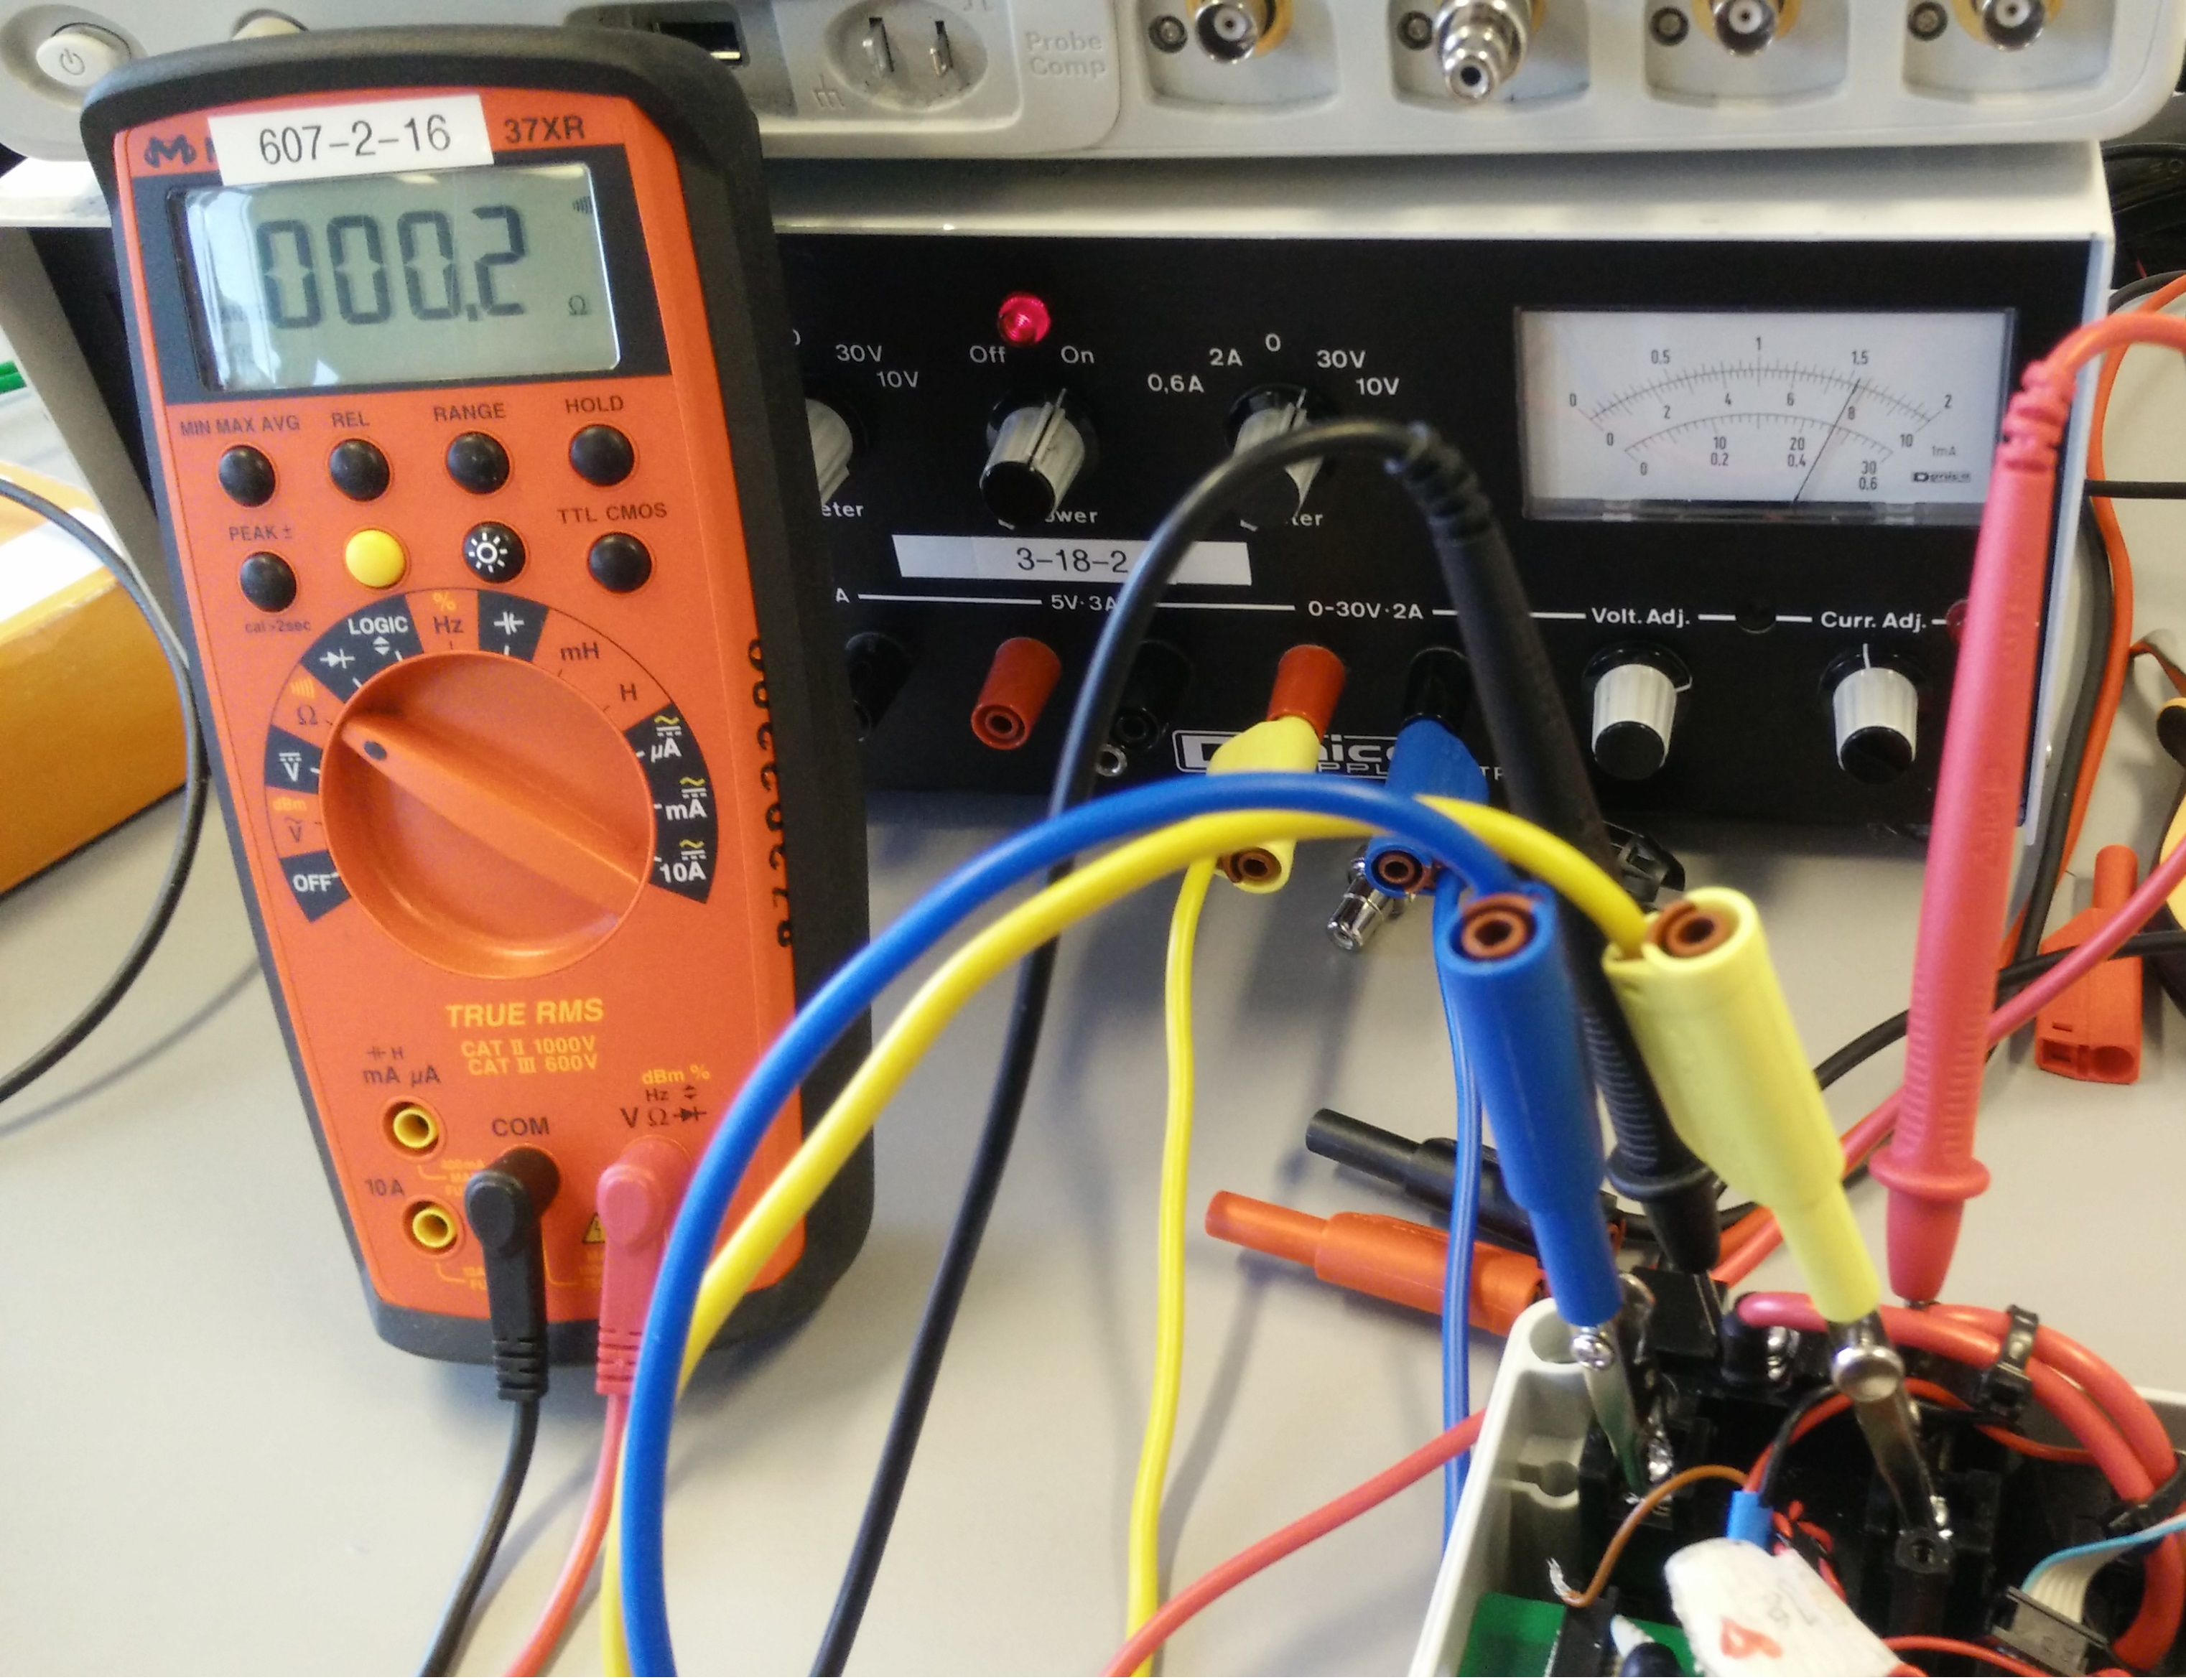
\includegraphics[width=1.0\linewidth]{Hardware/Pictures/BMSIsoTest}
	\caption[Empty]{Test setup for the test of the Isolation Switch relay.}
	\label{fig:BMSIsoTest}
\end{figure}


\subsubsection{Digital Unit (HW)}
The Digital Unit could be tested by analyzing the circuitry especially around the most critical parts to the Digital Unit. These include the USB interface circuit along with the F-RAM IC. The tests could include testing each of the pins of the IC and/or test the units separately by trying to exclude as much of the surrounding circuitry as possible. Investigating the parts around these would be a crucial step in finding a solution to the problem. Furthermore, if there are problems with connecting to the AVR-CAN board and more specifically the AT90CAN128 IC then this should be replaced. A procedure to test the software and program the BMS can be found in section \vref{sec:BMSDebugging}. However, there were no problems with the Digital Unit and it was working properly and as expected. Therefore no unit testing was required for the Digital Unit but some possible approaches have been listed. 

\subsubsection{Analog Front End}
The Analog Front End posed a lot of problems. These were tried to be resolved all the way to the end - before the hand-in. However, we were unsuccessful in getting the Analog Front End to function again.\\

\begin{figure}[H]
	\centering
	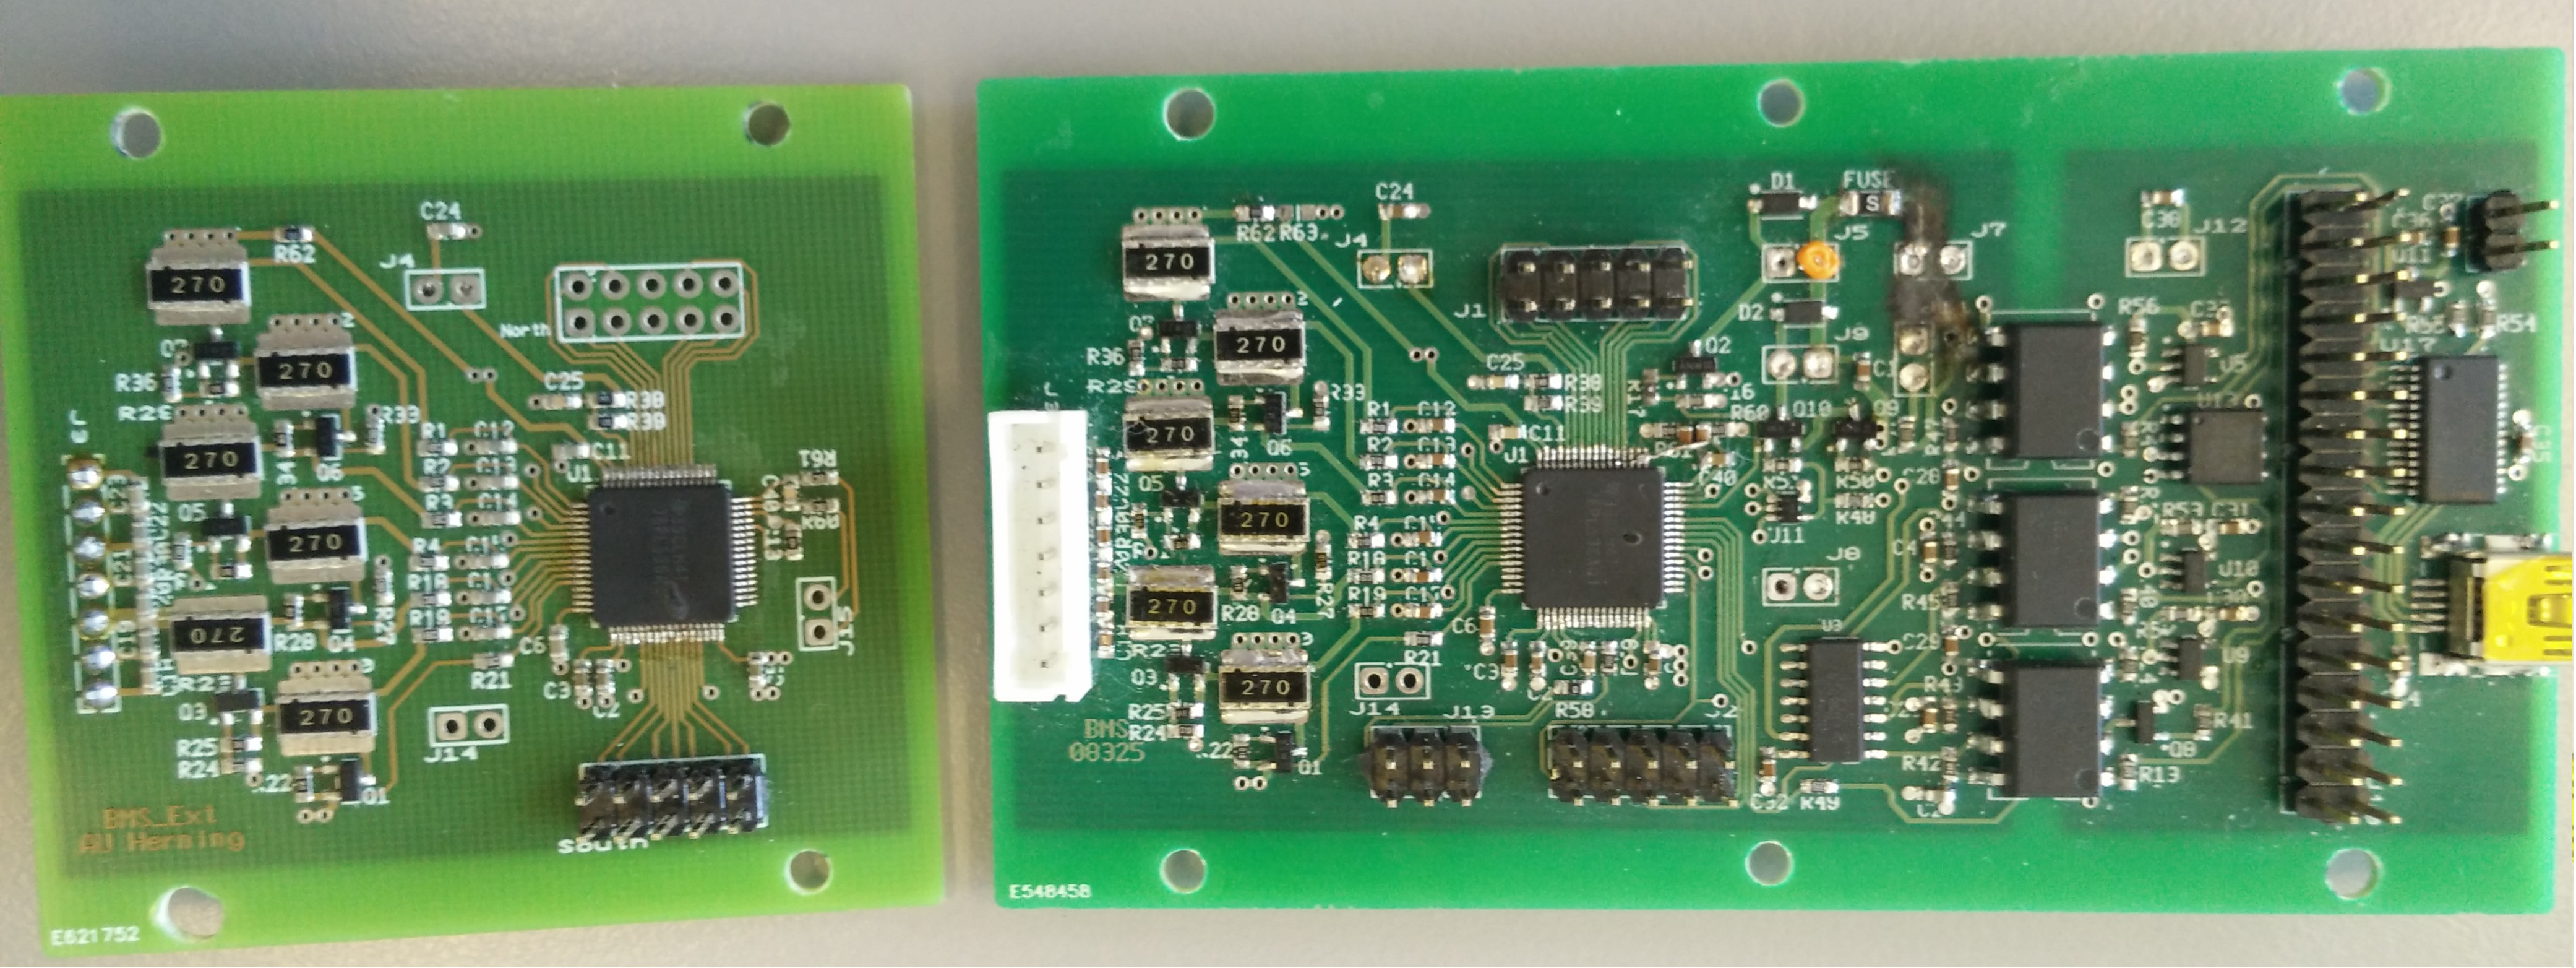
\includegraphics[width=1.0\linewidth]{Hardware/Pictures/BMSPCBS}
	\caption[Empty]{Picture of the PCBs of both the Analog Front End and the Extension Module.}
	\label{fig:BMSPCBS}
\end{figure}

Above on figure \vref{fig:BMSPCBS} you can see the PCBs of the Analog Front End along with the Extension Module. These are very complex and therefore very hard to debug, however it was still attempted. In this section a detailed walk through of what possible approaches have been taken and which could have been taken to solve the problem will be given. \\
The problem lies with the Battery Monitoring IC. The origin of this problem was that the Extension Module was wrongfully connected to the Analog Front End. This resulted in the Battery Monitor ICs on both the Extension Module and the Analog Front End were instantly fried. This happened when a shopping list for extra components to the duplicate prints was being developed. This led us to ordering several Battery Monitor ICs as well as a handful of additional components for backup if those were to break or be destroyed by the harsh conditions. Many measures were taken to ensure a fully functional Analog Front End, however, none of those succeeded. One of these were to simply desolved the broken IC and replace it with a new one. We expected that this would solve the problem, however, it didn't. Since we couldn't get any read out of the chip we meant that it was exposed more heat than it could handle during the soldering process. Therefore we had another pair soldered using a special SMD soldering machine. The result was the same we couldn't a connection established to the Analog Front End. When we were debugging with the USB interface we kept getting "CRC Errors", which is errors specified by the manufacturer of the Battery Monitor ICs. In the code this is specified as there's no connection to the chip from the Digital Unit. We had to conclude that the Battery Monitor IC was fully functional and therefore had to conclude that one or more components must have been fried along with the IC. \\
The next course of action was to approach the surrounding components. We meant that the transistors were the cause of the problem since one of them could easily have fried when the wrongful connection was made earlier. After testing the transistors with the diode test on a multimeter the problem still wasn't found. We resided to a hex-inverter located on the circuit but this wasn't documented in the old documentation \fxnote{reference to BMS 2013}. Therefore we didn't pursue the problem any further. Everything should be in working order, however, it wasn't.\\
The testing was done only with the Analog Front End, since we could factor out the Extension Module by only measuring on one battery and try to get a readout from that approach. The hours spent on debugging the Analog Front End as well as getting help from the School's workshop didn't result in any working condition of the Analog Front End. Therefore it was decided to focus on other things and let it be to try and find a solution before the departure for the Shell Eco-Marathon competition. \\


\subsubsection{Current Sensor}
The Current Sensor is meant to be functioning giving the first tests at a very early stage. However, the Analog Front End posed a lot of problem and those haven't been resolved even after very long hours of debugging. Therefore, it wasn't possible to test this unit. However, if the BMS was fully functional a way to test the current sensor would be to firstly identify the problem. Lets say we applied a constant current load of 4 Amps to the BMS. This would result in a specific result and data output from the Analog Front End. These data could then be examined by using the USB interface and confirm the values. If for instance different values were output the code for the calculation for the current sensor as well as individual components would need to be investigated. A good start would be to replace the OP-AMPs as well as the LDO since the rest of the components contained in the circuit \fxnote{reference til BMS 2013 current sensor} are merely passive components. Tests could be done for continuity and expected voltage levels in the circuit with a digital multimeter. These tests should be sufficient enough to test the current sensor since it is a rather small circuit with a basic functionality. In a worst case scenario a duplicate should be made on an entirely new PCB and then tested individually before being implemented into the BMS.    

\subsection{Programming Quick Guide}
\label{sec:BMSDebugging}
The purpose of this section is meant to help whoever is going to work with the BMS in the future. Here you will be guided in how to use, debug and program the Digital Unit thus the BMS.

Firstly, you will need a few prerequisites listed below to be able to program the BMS. Since the BMS was originally build in 2013 the software to program the BMS is outdated but sometimes it is only possible to proceed and get it to work with the specified utilities. 

Tools required to program the BMS are listed here:
	\begin{itemize}
		\item AVR Studio 4 (tested with version 4.19 Build 730).
		\item Atmel Studio 6 or 7 (Both tested).
		\item JTAG-USB programmer (programmer that is included with the BMS hardware).
		\item 2 batteries (used to power the BMS).
		\item Tera Term (or any other hyper terminal).
		\item USB-A to USB mini cable (used to debug the BMS and see readouts from Tera Term).
	\end{itemize}
	
After you have acquired these tools you are ready to proceed. First of you connect the USB cable from your computer to the BMS front end. Then you launch your chosen hyper terminal and select the COM-port which the BMS has. Afterwards you configure the hyper terminal, where the two most important settings are the baud rate and the way you receive from the BMS. Set the baud rate to 38400, 1 stop bit, 8 data bits and 0 parity bits. Then you specify the newline settings so that you receive both CR+LF else select AUTO. In Tera Term you go to Setup->Terminal->New-line to perform these changes. 
Now you can attach the two batteries to the BMS (remember to plug in both the main plug and the cell plug to the front end), once this is done you're ready to receive data from the front end whilst a successfull and working condition of the BMS USB interface should look something like in the figure below \vref{fig:BMSTeraTerm}. 
\begin{figure}[H]
	\centering
	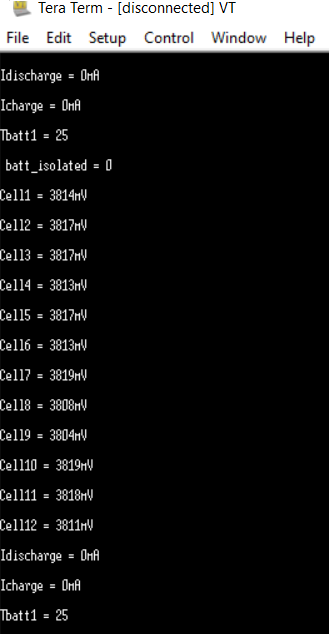
\includegraphics[width=0.6\linewidth]{Hardware/Pictures/BMS_teraterm}
	\caption{Tera Term Printout from BMS}
	\label{fig:BMSTeraTerm}
\end{figure}

\fxnote{referere to unit test }

Now you're ready to program the BMS. You can compile the code from either Atmel Studio 6 or 7, when you're done compiling you'll have a .hex file which is used for the AVR-CAN (Digital Unit). From this point on you have to follow the guide located in the pdf-file "How-to-install-and-use-AVR-JTAG-USB.pdf" which is located in the BMS repository. Now you can program the AVR-CAN module by selecting the .hex file or other valid files and program the BMS.

You can always confirm the programming by looking at the hyper terminal printouts and see if it matches your expectations. However, if it does not match your expectations you will have to debug the source code or the hardware to resolve the problem.

